\section{Vorbereitung auf den Versuch}

In diesem Versuch geht es darum, die Größe der Lichtgeschwindigkeit mithilfe der Drehspiegelmethode zu bestimmen (Abb. \ref{fig:Drehspiegelmethode}). Dafür wird ein Laserstrahl über einen Strahlenteiler geschickt, wobei dieser dahinter auf einen Drehspiegel trifft, der sich mit regulierbarer Frequenz dreht. Der Strahl durchquert eine Linse und trifft, nach einer weiteren Umlenken durch einen Spiegel, senkrecht auf einen Endspiegel. Der Strahlengang kehrt sich nun um, wobei sich der Drehspiegel in der Zwischenzeit um einen Winkel $\delta$ weitergedreht hat. Vom Strahlteiler wird dieser nun auf den Schirm geschickt.\\

\begin{figure}
    \centering
    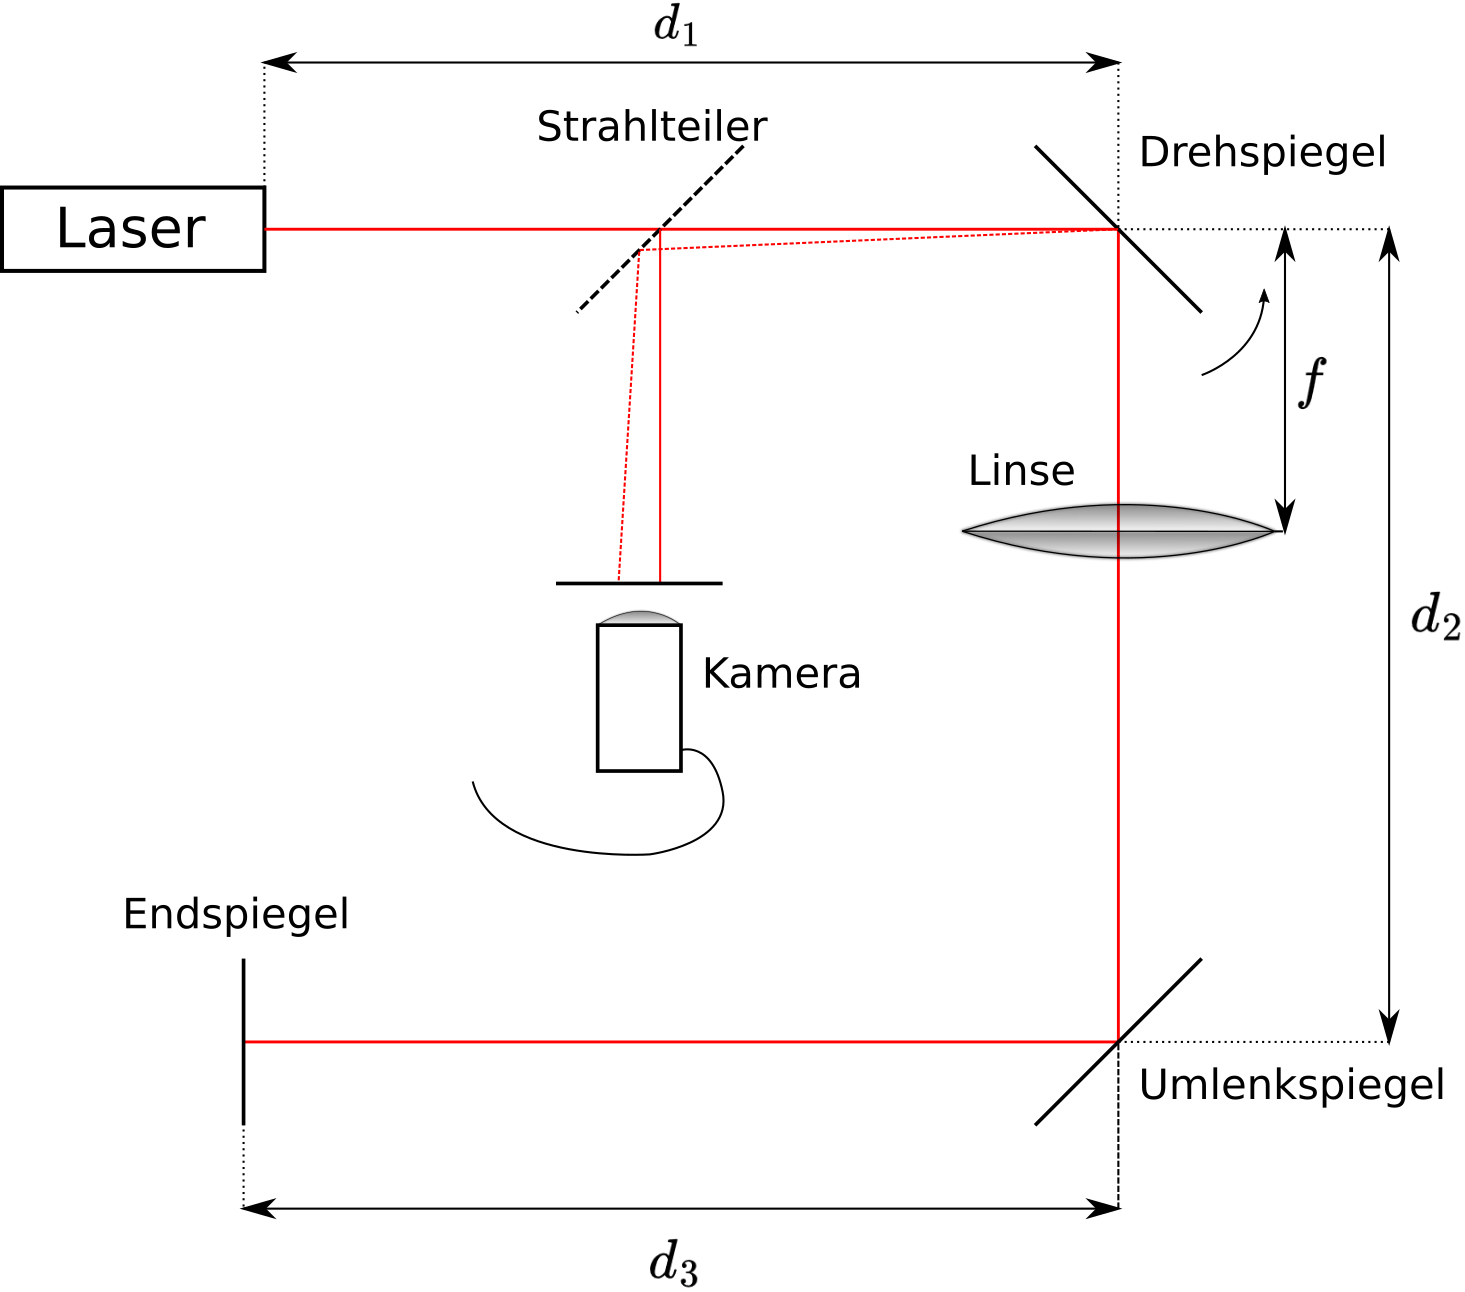
\includegraphics[scale=0.6]{Lichtgeschwindigkeit/Protokoll/fig/Drehspiegelmethode.png}
    \caption{Drehspiegelmethode}
    \label{fig:Drehspiegelmethode}
\end{figure}

Gemessen wird nun der Abstand a, also der Abstand zu dem Punkt, wo der Strahl bei ruhendem Drehspiegel auftreffen würde. Dieser wird auf der Millimeterskala auf dem Schirm für unterschiedliche Frequenzen gemessen.\\
Da der Versuch schon aufgebaut wurde, sind einige Werte, die für die Auswertung wichtig sind, schon gegeben. Diese sind in Tabelle \ref{tab:Drehspiegel vorgegebene Werte} aufgeführt.

\begin{table}[h]
    \centering
    \caption{Gegebene Werte Versuchsaufbau Drehspiegel}
    \begin{tabular}{c c c}
    \hline
    Abstand & Symbol & Wert \\
    \hline
    Laser-Drehspiegel Maximal & $d_{1max}$ & \SI{6.8}{\metre} \\
    Laser-Drehspiegel & $d_1$ & \SI{6.51}{\metre}\\
    Drehspiegel-Umlenkspiegel & $d_2$ & \SI{7.23}{\metre}\\
    Umlenkspiegel-Enspiegel & $d_3$ & \SI{6.59}{\metre}\\
    Brennweite Linse & $f$ & \SI{5}{\metre}\\
    
    \hline
    \end{tabular}
    \label{tab:Drehspiegel vorgegebene Werte}\\
    Fehler auf alle gegebenen Werte \SI{0.03}{\metre}.
\end{table}

Vorbereitend sollen nun die Positionen von Linse und Laseraustrittsöffnung berechnet werden. In diesem Versuchsaufbau wird eine Linse verwendet, damit der Strahl sowohl auf dem Dreh- als auch auf dem Enspiegel gebündelt wird und man somit ein scharfes Bild bekommt. Damit dies der Fall ist, muss der Abstand zwischen Drehspiegel und Linse gerade der Brennweite entsprechen. Um nun kann man sich die Gesetze der geometrischen Optik zu nutze machen \cite{2}. Man erhält durch Anwendung der Linsenleichung: 

\begin{equation}
    \frac{1}{f} = \frac{1}{b} + \frac{1}{g} = \frac{1}{d_1 + f} + \frac{1}{d_2 - f + d_3}
\end{equation}

Diese Formel wird nun nach $d_1$ umgestellt und man erhält:

\begin{equation}
    d_1 = \frac{f^2}{d_2+d_3-2f} \approx \SI{6.544}{\metre}
\end{equation}

Dieser Wert dient nur zur Überprüfung des voreingestellten Werts und dieser kann somit, da es nur eine kleine Abweichung gibt, übernommen werden.

Aus dem Abstand $a$ kann man nun auf die Lichtgeschwindigkeit schließen, die Formel dafür wird im folgenden hergeleitet:\\
Der Abstand a ist abhängig vom Winkel $\delta$, um den sich der Drehspiegel dreht, während das Licht den skizzierten Weg zurücklegt. Man erhält:

\begin{equation} \label{a}
    a = d_1 \tan{2\delta} \approx 2\delta d_1
\end{equation}

Man erhält nun weiter für die Zeitdifferenz $\Delta t$, die der Laserstrahl braucht:

\begin{equation}
    \Delta t = \frac{\delta}{\omega} = \frac{\delta}{2\pi f} \stackrel{(\ref{a})}{=} \frac{a}{4\pi f d_1}
\end{equation}

Und für die Streckendifferenz $\Delta s$:

\begin{equation}
    \Delta s = 2(d_2 + d_1)
\end{equation}

Der Wert für die Lichtgeschwindigkeit ergibt sich nun aus der Differenz von $\Delta s$ und $\Delta t$:

\begin{equation} \label{Drehspiegelmethode Formel}
    c = \frac{\Delta s}{\delta t} = \frac{8\pi f d_1 ( d_2 + d_3)}{a}
    \Rightarrow a = \frac{8 \pi f d_1 (d_2 + d_3)}{c}
\end{equation}

Es soll zusätzlich noch der erwartete Effekt berechnet werden, dafür werden die gegebenen Werte, zusammen mit dem Literaturwert für die Lichtgeschwindigkeit $c$ und einer Frequenz von $f = \SI{500}{\Hz}$ in die Formel \ref{Drehspiegelmethode Formel} eingesetzt und man erhält $a \approx \SI{0.00377}{\metre} = \SI{3.77}{\milli\metre}$.

\section{Justierung der Apparatur und Messung}

Die Justierung und das überprüfen der Positionen der Spiegel und der anderen Objekte enfiel, da der Versuch schon fertig aufgebaut vorgefunden wurde. Bei der Durchführung der Messungen wurde die Ablenkung a in Abhängigkeit von der Rotationsfrequenz des Drehspiegels notiert. Die Messwerte sind in Tabelle \ref{tab:Messwerte Drehspiegelmethode} aufgetragen.

\begin{table}[h]
    \centering
    \caption{Messwerte Drehspiegelmethode}
    \label{tab:Messwerte Drehspiegelmethode}
    \begin{tabular}{c c}
    \hline
    Rotationsgeschwindigkeit in $\frac{U}{m}$ & Lasserstrahlauftreffposition in $mm$ \\
    \hline
    1000 & 24.4 \\
    2000 & 24.5 \\
    3000 & 24.6 \\
    3950 & 24.7  \\
    4950 & 24.9 \\
    6000 & 25 \\
    6900 & 25.1\\
    8000 & 25.2 \\
    9050 & 25.3 \\
    10000 & 25.4 \\
    11000 & 25.4 \\
    12020 & 25.6 \\
    12970 & 25.9 \\
    13950 & 26 \\
    15000 & 26.1 \\
    \hline
    \end{tabular}
\end{table}

\section{Auswertung}

Die Formel \ref{Drehspiegelmethode Formel} lässt sich so umschreiben, dass man direkt die Drehzahl des Rotationsspiegels U einsetzen kann: 

\begin{equation} \label{Drehspiegelmethode Formel Drehzahl}
    a = \frac{8 \pi  d_1 (d_2 + d_3)}{60c} U
\end{equation}

Mit dieser Formel und den Messdaten aus Tabelle \ref{tab:Messwerte Drehspiegelmethode} wird nun eine lineare Regression durchgeführt (Abb. \ref{fig:Drehspiegelmethode Anpassung} )

Für die Steigung ergibt sich somit: 
\begin{equation} \label{Steigung Drehspiegelmethode}
    m = \frac{8 \pi  d_1 (d_2 + d_3)}{60c} = 8290 \, \frac{1}{mm\cdot s}
\end{equation}

Durch Umformung der Gleichung \ref{Drehspiegelmethode Formel Drehzahl} und einsetzen von m erhält man:

\begin{equation}
    c = m \frac{8 \pi d_1 (d_2+d_2)}{60}  \stackrel{(\ref{Steigung Drehspiegelmethode})}{\Rightarrow} c = \SI{287940287.054}{\metre\per\second}
\end{equation}

\begin{figure}[ht]
    \centering
    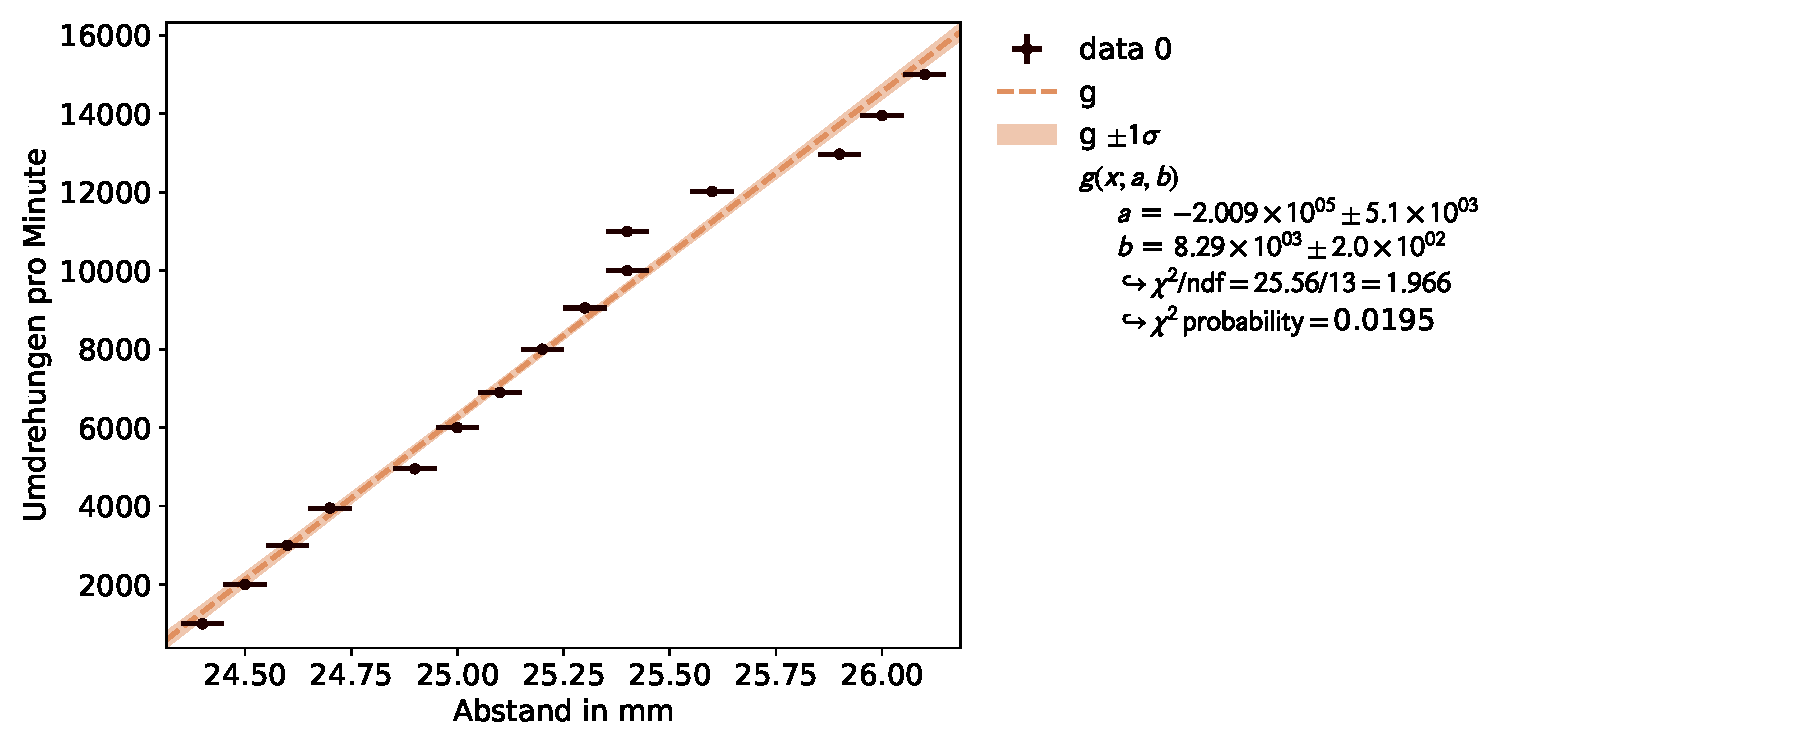
\includegraphics[scale=0.45]{Lichtgeschwindigkeit/Protokoll/fig/Drehspiegelmethode.pdf}
    \caption{Lineare Regression Drehspiegelmethode}
    \label{fig:Drehspiegelmethode Anpassung}
\end{figure}

\section{Fehlerrechnung}

\subsection{Statistischer Fehler}

Den statistischen Fehler entnehmen wir dem Plot. Somit erhält man einen von Kafe2 bestimmten Fehler auf die Steigung von $\pm 200 \, \frac{1}{mm \cdot s}$. Den statistischen Fehler auf die berechnete Lichtgeschwindigkeit erhält man nun durch die Gaußsche Fehlerfortpflanzung:

\begin{equation}
    \sigma_{c_{stat}} = \sqrt{(\frac{\partial c }{\partial m})^2 \sigma_m^2} = \sqrt{( \frac{8 \pi d_1 (d_2+d_2)}{60})^2 \sigma_m^2} \approx \SI{7706226}{\metre\per\second}
\end{equation}

Wie man erkennen kann, ist die statistische Abweichung größer als die Abweichung zum Literaturwert. Also müssen auch die systematischen eine signifikante Rollte spielen. 

\subsection{Systematischer Fehler}

Mögliche Fehlerquellen sind zum Beispiel:
\begin{itemize}
    \item Skala zum Ablesen der Laserpunktposition
    \item Bestimmung der Positionen der Spiegel und anderer Objekte
    \item Frequenzbestimmung des Drehspiegels
\end{itemize}

Zur Berechnung des systematischen Fehlers wird die Formel für die Größtfehlerabschätzung verwendet. Für die Lichtgeschwindigkeit gilt nach Gleichung \ref{Drehspiegelmethode Formel Drehzahl}:

\begin{equation}
    c = \frac{8 \pi  d_1 (d_2 + d_3)}{60a} U
\end{equation}

Damit ergibt sich für die Größtfehlerabschätzung:

\begin{align}
    \Delta_c &= \Bigl| \frac{\partial c}{\partial U} \Bigl| \Delta_U + \Bigl|
    \frac{\partial c}{\partial d_1} \Bigl| \Delta_{d_1} + \Bigl| \frac{\partial
    c}{\partial d_2} \Bigl| \Delta_{d_2} + \Bigl| \frac{\partial c}{\partial d_3}
    \Bigl| \Delta_{d_3} + \Bigl| \frac{\partial c}{\partial a} \Bigl| \Delta_a \\
    \Delta_c &= 8 \pi d_1 \frac{d_2 + d_3}{60a}\Delta U + 8 \pi U \frac{d_2 + d_3}{60a}\Delta d_1 + 8 \pi U d_1 \frac{1}{60a} \Delta d_2 + 8 \pi U d_1 \frac{1}{60a} \Delta d_3 + 8 \pi U d_1 \frac{d_2 + d_3 }{60a^2} \Delta a \\
    \Delta_c &= \SI{4030775.874}{\metre\per\second}
\end{align}

\subsection{Messergebnis}

Mithilfe der berechneten Werte, kann man nun das Messergebnis angeben:

\begin{align}
    c_{ges} &= c \pm \sigma_c \pm \Delta_c \\
    c_{ges} &= \SI{287940287.054}{\metre\per\second} \pm \SI{7706226}{\metre\per\second} \pm  \SI{4030775.874}{\metre\per\second}\\
    c_{ges} &= \SI{287940287.054 \pm 11737001.87}{\metre\per\second} \\
     c_{ges} &= \SI{287940287.054}{\metre\per\second} \pm 4.07 \%
\end{align}

Der Literaturwert beläuft sich auf $c_0 = 2.998 \cdot 10^8 \, \frac{m}{s}$, somit liegt der Literaturwert innerhalb unserer Fehlergrenzen.
Ein zufriedenstellendes Ergebnis